\chapter{Methodologies}

In the IT context, a methodology refers to a structured approach or set of principles and practices that guide the planning, development, implementation, and management of IT projects or processes. It provides a systematic framework for organizing and executing tasks, as well as a common language and set of tools to facilitate collaboration among team members. A methodology encompasses a range of activities, techniques, and guidelines tailored to address specific challenges and ensure successful outcomes in IT projects.

A methodology typically outlines a step-by-step process for undertaking IT initiatives, including project initiation, requirements gathering, design, development, testing, deployment, and maintenance. It may incorporate various methodologies or frameworks, such as Agile, Waterfall, Scrum, or Lean, depending on the specific needs of the project. The choice of methodology often depends on factors such as project size, complexity, team structure, and organizational culture.

A well-defined methodology brings several benefits to the IT context. It promotes consistency and standardization in project execution, allowing for more predictable outcomes and better resource management. It helps identify and mitigate risks early in the project lifecycle, facilitating proactive decision-making. Additionally, a methodology supports effective communication and collaboration among project stakeholders, ensuring shared understanding and alignment of objectives. By providing a structured approach, a methodology enhances project transparency, facilitates progress tracking, and enables continuous improvement through feedback and lessons learned.

{\Large Add something about SIX SIGMA}

\section{Agile}

\href{https://www.atlassian.com/agile/manifesto}{Source!}\\

\begin{center}
	{\Large Manifesto for Agile Software Development}\\
We are uncovering better ways of developing software by doing it and helping others do it.\\

Through this work we have come to value:\\

\textbf{Individuals and interactions} over processes and tools\\

\textbf{Working software} over comprehensive documentation\\

\textbf{Customer collaboration} over contract negotiation\\

\textbf{Responding to change} over following a plan\\

That is, while there is value in the items on the right, we value the items on the left more.
\end{center}

Agile is an iterative and collaborative approach that focuses on flexibility and adaptability. It emphasizes frequent communication, incremental development, and delivering working software in short iterations.

\subsection{Scrum}

Scrum is an Agile framework that utilizes cross-functional teams to deliver software incrementally. It involves iterative sprints, daily stand-up meetings, and continuous collaboration to foster flexibility and rapid development.

\subsection{Kanban}

Kanban is a visual project management approach that focuses on continuous delivery and workflow optimization. It uses a Kanban board to visualize tasks, limit work in progress, and optimize the flow of work.


\section{Waterfall - measure twice, cut once}
\href{https://business.adobe.com/blog/basics/waterfall#:~:text=The%20waterfall%20methodology%20is%20a,detailed%20documentation%2C%20and%20consecutive%20execution.}{Source!}\\

Waterfall is a sequential and linear approach where each phase of a project is completed before moving to the next one. It follows a structured process with defined milestones, making it suitable for projects with well-defined requirements and minimal changes.

In other words, the waterfall methodology is a project management approach that emphasizes a linear progression from beginning to end of a project. This methodology, often used by engineers, is front-loaded to rely on careful planning, detailed documentation, and consecutive execution.

The Waterfall methodology — also known as the Waterfall model — is a sequential development process that flows like a waterfall through all phases of a project (analysis, design, development, and testing, for example), with each phase completely wrapping up before the next phase begins.

It is said that the Waterfall methodology follows the adage to “measure twice, cut once.” The success of the Waterfall method depends on the amount and quality of the work done on the front end, documenting everything in advance, including the user interface, user stories, and all the features’ variations and outcomes.

\subsection{5 common stages in a Waterfall process}

The Waterfall methodology follows a chronological process and works based on fixed dates, requirements, and outcomes. With this method, the individual execution teams aren’t required to be in constant communication and, unless specific integrations are required, are usually self-contained.

Team members also tend to work independently and aren’t expected to provide status reports as often as with the Agile approach. Usually, one phase doesn’t begin until the previous one is finished.

%\begin{figure}[h]
%	\centering
%	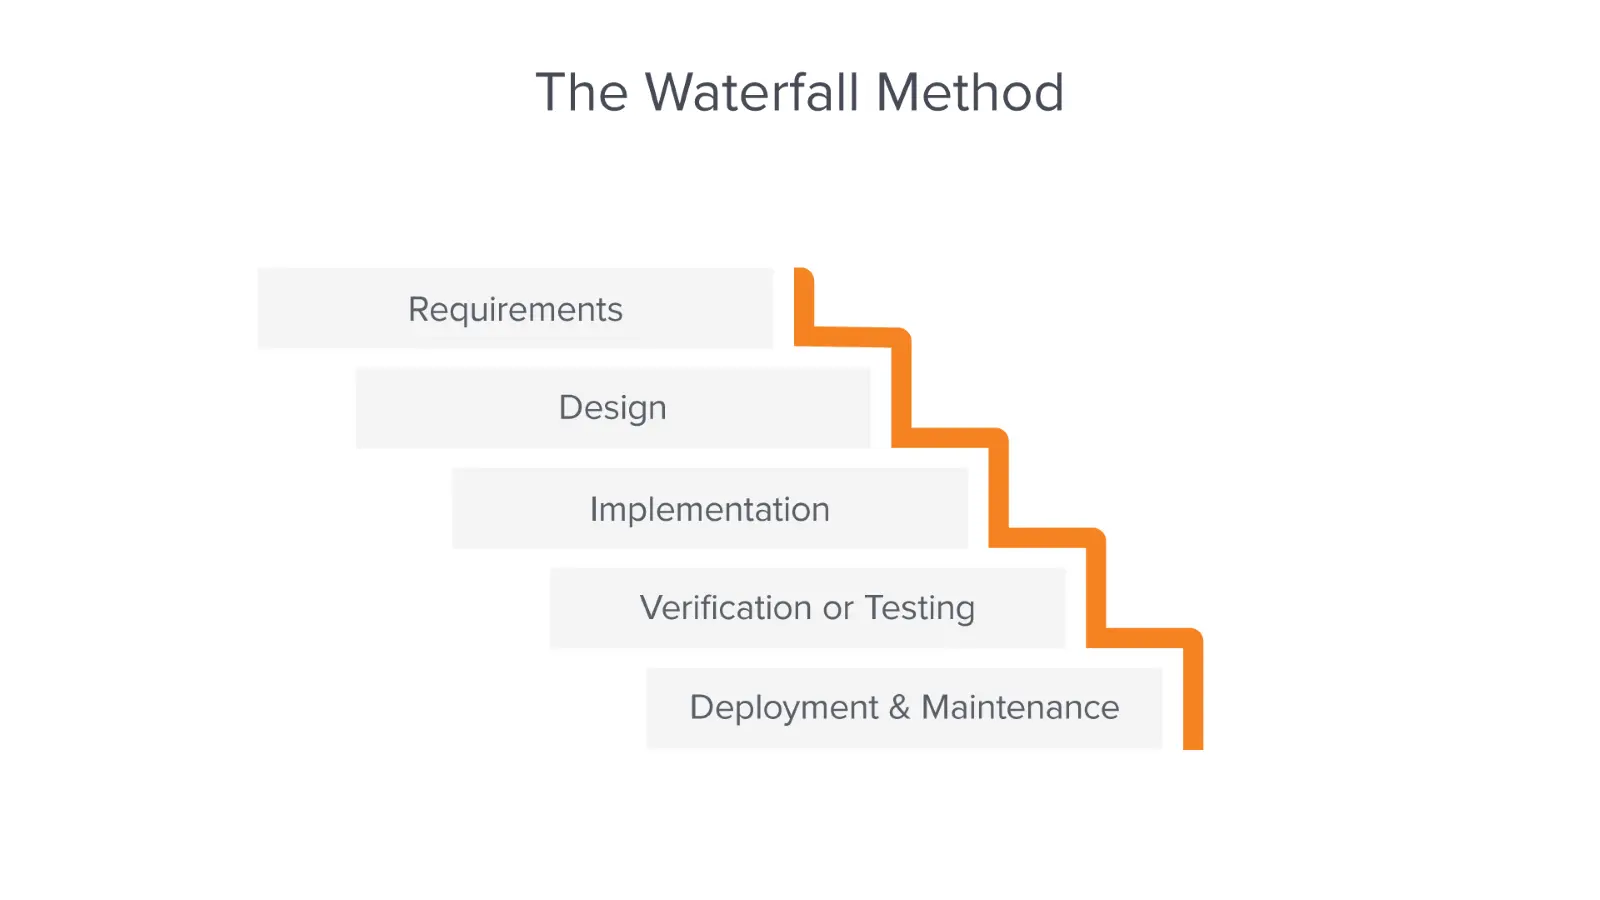
\includegraphics[scale=0.20]{./images/chapter_1_img_1.jpg}
%	\caption{Waterfall stages}
%\end{figure}

\subsubsection{Requirements}
\subsubsection{Design}
\subsubsection{Implementation}
\subsubsection{Verification or Testing}
\subsubsection{Deployment \& Maintenance}

\section{Lean}

Lean methodology aims to eliminate waste and maximize value in the software development process. It emphasizes continuous improvement, customer focus, and efficient resource utilization.

\section{DevOps}

DevOps combines software development (Dev) and IT operations (Ops) to enhance collaboration and streamline the software delivery lifecycle. It focuses on automation, continuous integration, continuous delivery, and close collaboration between development and operations teams.

\section{Rapid Application Development (RAD)}

RAD is a methodology that emphasizes rapid prototyping and iterative development. It involves user feedback and frequent iterations to quickly build and refine software applications.

\section{Extreme Programming (XP)}

XP is an Agile methodology that emphasizes close collaboration, continuous feedback, and a high degree of customer involvement. It emphasizes practices like test-driven development, pair programming, and frequent releases.

\section{Spiral}

The Spiral methodology is a risk-driven approach that combines elements of both waterfall and iterative development. It involves iterative cycles where the project progresses through planning, risk analysis, prototyping, and customer evaluation.

\section{Feature-Driven Development (FDD)}

FDD is an iterative and incremental methodology focused on delivering tangible features quickly. It emphasizes domain modeling, iterative development, and feature-level planning and tracking.